\documentclass[11pt,a4paper]{article}

\usepackage[margin=1in]{geometry}
\usepackage{amsmath}
\usepackage{booktabs}
\usepackage{graphicx}
\usepackage{hyperref}
\usepackage{xcolor}

\graphicspath{{../}}
\hypersetup{
    colorlinks=true,
    linkcolor=blue,
    urlcolor=blue,
    citecolor=blue
}

\title{DQN with Schmidhuber-Style Curiosity\\
       Experiment Report}
\author{Curious-Agent-RL}
\date{28 July 2026}

\begin{document}

\maketitle

\begin{abstract}
This report presents the results of training a Deep Q-Network (DQN) agent
with a Schmidhuber-style intrinsic curiosity signal in a heterogeneous
$10\times10$ grid world. An initial environment implementation prevented the
controller from influencing transitions because zone dynamics replaced the
selected action. The environment was corrected so that every transition begins
with the selected action and the zone dynamics subsequently modify its result.
After this correction, the DQN learned to reach the external goal consistently:
the average total reward over the final 100 episodes was $1.004$, average
curiosity reward was $0.004$, and mean episode length near the end of training
was approximately $21$ steps. These results demonstrate successful task
learning, although further ablation studies are required to isolate the
contribution of curiosity.
\end{abstract}

\section{Introduction}

The experiment is inspired by Schmidhuber's curious model-building control
systems. The agent contains three learned components:

\begin{enumerate}
    \item a world model $M$ that predicts the next state;
    \item a confidence model $C$ that predicts the world model's error; and
    \item a DQN controller $Q$ that selects actions using the sum of external
          and intrinsic rewards.
\end{enumerate}

The intrinsic reward is intended to represent learning progress. In the current
implementation it is calculated as

\begin{equation}
    r^{\mathrm{cur}}_t =
    C_{\mathrm{before}}(s_t,a_t) -
    C_{\mathrm{after}}(s_t,a_t),
\end{equation}

and the controller receives

\begin{equation}
    r^{\mathrm{total}}_t =
    r^{\mathrm{ext}}_t + \beta r^{\mathrm{cur}}_t,
\end{equation}

where $\beta=1.0$ in the reported experiment.

\section{Environment}

The environment is a $10\times10$ grid with four actions: up, down, left, and
right. The agent starts in the upper-left cell, while the external goal is in
the lower-right cell and provides a reward of $+1$. An episode terminates when
the goal is reached or after 200 steps.

The grid contains the zone distribution shown in
Table~\ref{tab:zones}. Zone modifiers are applied after the agent's intended
movement, ensuring that the transition remains action-dependent.

\begin{table}[ht]
    \centering
    \caption{Grid-world zone configuration after the controllability fix.}
    \label{tab:zones}
    \begin{tabular}{lll}
        \toprule
        Zone & Proportion & Transition behavior \\
        \midrule
        Static          & 10\% & Selected action only \\
        Deterministic A & 30\% & Action followed by an upward shift \\
        Deterministic B & 20\% & Action followed by a rightward shift \\
        Noisy           & 20\% & Action followed by a random local perturbation \\
        Dynamic         & 20\% & Action followed by a periodically changing shift \\
        \bottomrule
    \end{tabular}
\end{table}

\subsection{Controllability correction}

In the original implementation, every configured zone replaced the selected
action. Static cells were absorbing, deterministic cells moved according to a
fixed rule, and noisy cells teleported to a random grid location. Because the
configured zones occupied all grid cells, the action chosen by the DQN had no
meaningful effect on the transition.

The corrected transition is

\begin{equation}
    \tilde{s}_{t+1} = f_{\mathrm{action}}(s_t,a_t),
    \qquad
    s_{t+1} = f_{\mathrm{zone}}(\tilde{s}_{t+1}).
\end{equation}

Static cells apply no additional modifier, deterministic and dynamic cells add
their respective shifts, and noisy cells add a local stochastic perturbation.
This makes action values identifiable while retaining heterogeneous dynamics.

\section{DQN Configuration}

The principal training settings are summarized in
Table~\ref{tab:training-config}.

\begin{table}[ht]
    \centering
    \caption{DQN training configuration.}
    \label{tab:training-config}
    \begin{tabular}{lr}
        \toprule
        Parameter & Value \\
        \midrule
        Training episodes & 2000 \\
        Maximum steps per episode & 200 \\
        Discount factor $\gamma$ & 0.99 \\
        Curiosity weight $\beta$ & 1.0 \\
        Initial epsilon & 1.0 \\
        Epsilon decay per episode & 0.9995 \\
        Final epsilon & 0.368 \\
        Replay-buffer capacity & 10000 \\
        Replay warm-up & 1000 transitions \\
        Batch size & 64 \\
        Q-network learning rate & 0.001 \\
        World-model learning rate & 0.001 \\
        Confidence-model learning rate & 0.0005 \\
        Random seed & 42 \\
        \bottomrule
    \end{tabular}
\end{table}

The controller uses a dueling DQN architecture with two 128-unit hidden layers.
The world model has two 64-unit hidden layers, and the confidence network has
two 32-unit hidden layers. Metrics in the training log are averages over
non-overlapping windows of 10 episodes.

\section{Results}

Figure~\ref{fig:training-curves} presents the corrected training curves.
Reward increases toward $1.0$, episode length falls substantially, and
curiosity approaches a small value around zero. Epsilon remains relatively
high because it is decayed once per episode.

\begin{figure}[ht]
    \centering
    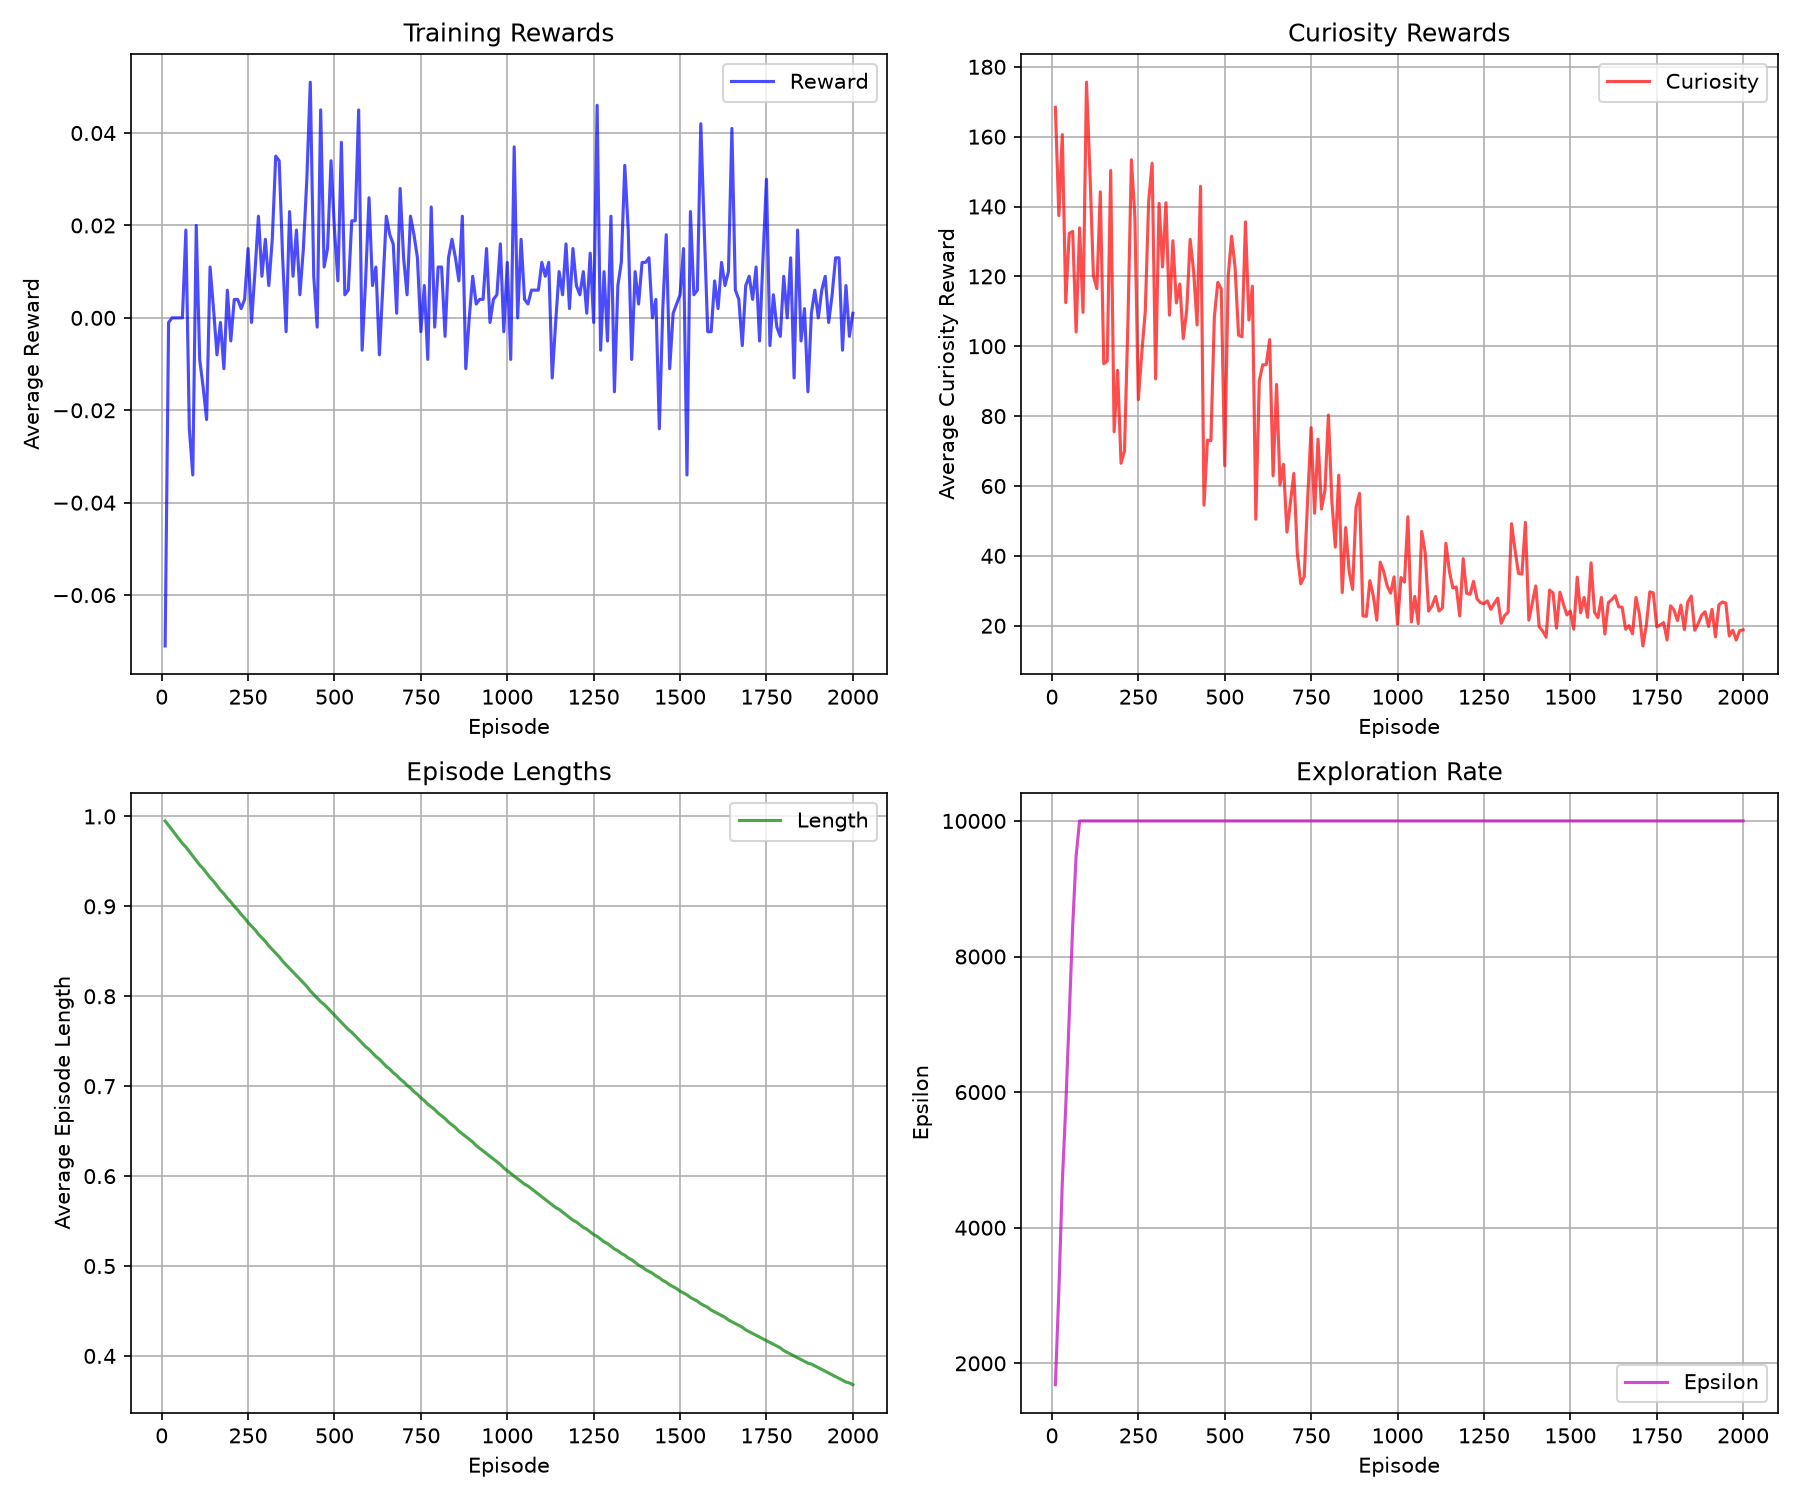
\includegraphics[width=\textwidth]{training_curves.png}
    \caption{DQN training reward, curiosity reward, episode length, and
    epsilon. Each point summarizes 10 episodes.}
    \label{fig:training-curves}
\end{figure}

Table~\ref{tab:window-results} summarizes several phases of training. External
reward is estimated as total reward minus curiosity reward because $\beta=1$.
Values following the $\pm$ symbol are population standard deviations across
the logged 10-episode windows.

\begin{table}[ht]
    \centering
    \caption{Training performance by episode range.}
    \label{tab:window-results}
    \begin{tabular}{lrrrr}
        \toprule
        Episodes & Total reward & Curiosity & Est.\ external reward
                 & Episode length \\
        \midrule
        10--200
            & $0.588\pm0.194$ & $-0.0072\pm0.0196$
            & $0.595\pm0.191$ & $123.7\pm29.3$ \\
        210--500
            & $0.692\pm0.185$ & $0.0157\pm0.0134$
            & $0.677\pm0.184$ & $111.5\pm26.1$ \\
        510--1000
            & $0.926\pm0.115$ & $0.0102\pm0.0114$
            & $0.916\pm0.119$ & $62.2\pm31.7$ \\
        1010--1500
            & $1.001\pm0.027$ & $0.0067\pm0.0123$
            & $0.994\pm0.024$ & $29.6\pm8.3$ \\
        1510--2000
            & $1.003\pm0.023$ & $0.0055\pm0.0126$
            & $0.998\pm0.014$ & $23.1\pm4.9$ \\
        1900--2000
            & $1.004\pm0.006$ & $0.0038\pm0.0063$
            & $1.000\pm0.000$ & $20.9\pm4.0$ \\
        \bottomrule
    \end{tabular}
\end{table}

\section{Discussion}

\subsection{Task performance}

The results provide strong evidence of successful task learning. Early in
training, estimated external reward was approximately $0.60$ and episodes
required about 124 steps on average. During the final 500 episodes, estimated
external reward increased to approximately $1.00$ while average episode length
fell to 23 steps. In the final logged windows the goal was reached consistently,
despite the behavior policy retaining an epsilon of $0.368$.

The reward curve contains substantial variation during the first 700 episodes.
This is expected from high epsilon-greedy exploration, stochastic noisy zones,
the changing intrinsic reward, and replay-buffer learning. The later reward
curve is stable around $1.0$, indicating convergence rather than collapse or
unbounded value growth.

\subsection{Curiosity behavior}

The curiosity signal does not decrease monotonically. It begins with a negative
transient, becomes positive while the predictive models are learning, and then
fluctuates close to zero. Its mean falls from approximately $0.016$ during
episodes 210--500 to approximately $0.006$ during the final 500 episodes.
Occasional positive and negative spikes are plausible in noisy and dynamic
zones: positive values indicate a decrease in predicted error, while negative
values indicate an increase.

A small late-stage curiosity reward is consistent with diminished learning
progress after predictable transitions have been learned. It should not,
however, be interpreted as proof that the confidence model accurately measures
world-model improvement.

\section{Limitations}

The experiment supports the conclusion that the corrected DQN learns the task,
but it does not yet establish that curiosity improves performance. Important
limitations include:

\begin{itemize}
    \item only one random seed is represented;
    \item there is no external-only DQN comparison with $\beta=0$;
    \item logged reward combines external and intrinsic rewards;
    \item evaluation is performed during training with nonzero epsilon;
    \item noisy and dynamic transitions make individual runs variable;
    \item historical intrinsic rewards stored in replay become stale as the
          predictive models change;
    \item the maintained target Q-network is not currently used to calculate
          the bootstrap target; and
    \item the current before/after confidence update is an approximation to
          world-model learning progress.
\end{itemize}

\section{Recommended Follow-up Experiments}

The next evaluation should compare at least the following conditions:

\begin{enumerate}
    \item DQN with curiosity ($\beta=1$);
    \item the same DQN without curiosity ($\beta=0$); and
    \item a random-policy baseline.
\end{enumerate}

Each condition should be repeated over at least five seeds. After training,
policies should be evaluated with epsilon set to zero, reporting success rate,
external return, and episode length separately. Confidence intervals should be
reported across seeds. Zone visitation and world-model prediction error should
also be logged to determine whether curiosity changes exploration rather than
merely adding a small reward perturbation.

\section{Conclusion}

Correcting the environment so that actions influence transitions transformed
the previously unsuccessful experiment into a convergent one. The DQN achieves
approximately one unit of external reward per episode near the end of training
and reduces average episode length from more than 120 steps to approximately
21--23 steps. Curiosity becomes small and approximately stable as learning
progress diminishes. Therefore, the experiment demonstrates satisfactory DQN
task learning. A multi-seed, curiosity-free ablation is still required before
claiming that the intrinsic reward itself improves learning.

\section*{Reproduction}

From the project root, train and generate the plot with:

\begin{verbatim}
venv/bin/python main.py --agent dqn
venv/bin/python -m scripts.visualize \
  --config configs/dqn.yaml \
  --mode curves \
  --log-file training_dqn.log
\end{verbatim}

Compile this report from the documentation directory:

\begin{verbatim}
cd docs
pdflatex report.tex
pdflatex report.tex
\end{verbatim}

\end{document}
